\begin{figure}[t]
    \centering
    \resizebox{0.98\textwidth}{!}{%
    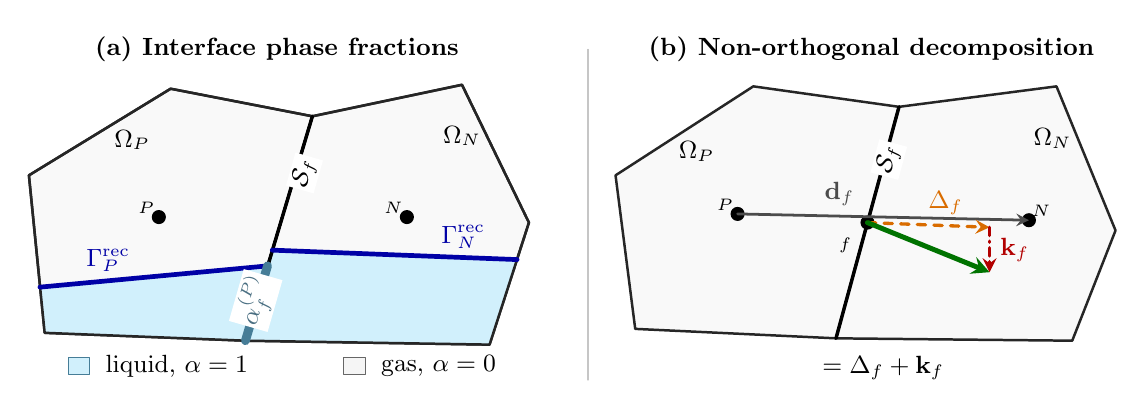
\begin{tikzpicture}[
        x=1cm,
        y=1cm,
        line cap=round,
        line join=round,
        >=stealth,
        every node/.style={font=\small},
        centre/.style={circle,fill=black,inner sep=1.8pt},
        cell/.style={draw=black!85,line width=0.9pt,fill=gray!5}
    ]
        % Panel (a): interface geometry and geometrical phase fractions.
        \begin{scope}
            \node[font=\small\bfseries] at (2.8,3.85)
                {(a) Interface phase fractions};

            \path[cell]
                (-0.15,0.25)--(2.40,0.15)--(3.25,3.00)--
                (1.45,3.35)--(-0.35,2.25)--cycle;
            \path[cell]
                (2.40,0.15)--(5.50,0.10)--(6.00,1.65)--
                (5.15,3.40)--(3.25,3.00)--cycle;

            \begin{scope}
                \clip
                    (-0.15,0.25)--(2.40,0.15)--(3.25,3.00)--
                    (1.45,3.35)--(-0.35,2.25)--cycle;
                \fill[cyan!18]
                    (-0.6,-0.2)--(6.2,-0.2)--(6.2,1.42)--
                    (2.68,1.10)--(-0.6,0.80)--cycle;
            \end{scope}
            \begin{scope}
                \clip
                    (2.40,0.15)--(5.50,0.10)--(6.00,1.65)--
                    (5.15,3.40)--(3.25,3.00)--cycle;
                \fill[cyan!18]
                    (-0.6,-0.2)--(6.2,-0.2)--(6.2,1.16)--
                    (2.74,1.30)--(-0.6,1.43)--cycle;
            \end{scope}

            % Redraw the cell boundaries over the phase fill.
            \draw[black!85,line width=0.9pt]
                (-0.15,0.25)--(2.40,0.15)--(3.25,3.00)--
                (1.45,3.35)--(-0.35,2.25)--cycle;
            \draw[black!85,line width=0.9pt]
                (2.40,0.15)--(5.50,0.10)--(6.00,1.65)--
                (5.15,3.40)--(3.25,3.00)--cycle;
            \draw[black,line width=1.25pt] (2.40,0.15)--(3.25,3.00);

            \draw[blue!65!black,line width=1.7pt]
                (-0.21,0.83)--(2.68,1.10)
                node[pos=0.30,above=-1pt] {$\Gamma_P^{\mathrm{rec}}$};
            \draw[blue!65!black,line width=1.7pt]
                (2.74,1.30)--(5.85,1.18)
                node[pos=0.78,above=-1pt] {$\Gamma_N^{\mathrm{rec}}$};
            \draw[cyan!55!black,line width=3.2pt]
                (2.40,0.15)--(2.68,1.10);

            \node[centre] at (1.30,1.72) {};
            \node[anchor=south east,inner sep=0pt,xshift=-1pt,yshift=1pt]
                at (1.30,1.72) {$\x_P$};
            \node[centre] at (4.45,1.72) {};
            \node[anchor=south east,inner sep=0pt,xshift=-1pt,yshift=1pt]
                at (4.45,1.72) {$\x_N$};
            \node at (0.96,2.70) {$\Omega_P$};
            \node at (5.15,2.75) {$\Omega_N$};
            \node[rotate=74,fill=white,inner sep=1pt] at (3.15,2.28)
                {$\mathcal S_f$};
            \node[rotate=74,fill=white,inner sep=0.8pt,
                text=cyan!45!black] at (2.53,0.66) {$\alpha_f^{(P)}$};
            \fill[cyan!18,draw=cyan!55!black] (0.15,-0.28) rectangle (0.42,-0.06);
            \node[anchor=west] at (0.50,-0.17) {liquid, $\alpha=1$};
            \fill[gray!8,draw=black!60] (3.65,-0.28) rectangle (3.92,-0.06);
            \node[anchor=west] at (4.00,-0.17) {gas, $\alpha=0$};
        \end{scope}

        % Panel divider.
        \draw[gray!45] (6.75,-0.35)--(6.75,3.85);

        % Panel (b): owner-neighbour geometry and non-orthogonal decomposition.
        \begin{scope}[xshift=7.35cm]
            \node[font=\small\bfseries] at (3.0,3.85)
                {(b) Non-orthogonal decomposition};

            \path[cell]
                (0.0,0.30)--(2.55,0.18)--(3.35,3.12)--
                (1.50,3.38)--(-0.25,2.25)--cycle;
            \path[cell]
                (2.55,0.18)--(5.55,0.15)--(6.10,1.55)--
                (5.35,3.38)--(3.35,3.12)--cycle;
            \draw[black,line width=1.25pt] (2.55,0.18)--(3.35,3.12);

            \coordinate (P) at (1.30,1.76);
            \coordinate (N) at (5.00,1.68);
            \coordinate (F) at (2.95,1.65);
            \coordinate (D) at (4.50,1.59);
            \coordinate (S) at (4.50,1.02);

            \node[centre] at (P) {};
            \node[anchor=south east,inner sep=0pt,xshift=-1pt,yshift=1pt]
                at (P) {$\x_P$};
            \node[centre] at (N) {};
            \node[anchor=south west,inner sep=0pt,xshift=1pt,yshift=1pt]
                at (N) {$\x_N$};
            \node[centre,label=below left:$\x_f$] at (F) {};
            \node at (0.78,2.55) {$\Omega_P$};
            \node at (5.3,2.72) {$\Omega_N$};
            \node[rotate=75,fill=white,inner sep=1pt] at (3.22,2.45)
                {$\mathcal S_f$};

            \draw[->,black!70,line width=1.0pt]
                (P)--(N) node[pos=0.35,above=0pt] {$\mathbf d_f$};
            \draw[->,orange!85!black,dashed,line width=1.2pt]
                (F)--(D) node[pos=0.64,above=0pt] {$\boldsymbol{\Delta}_f$};
            \draw[->,green!45!black,line width=1.8pt]
                (F)--(S) node[pos=0.64,below=3pt] {$\Sf$};
            \draw[->,red!70!black,dash dot,line width=1.2pt]
                (D)--(S) node[midway,right] {$\mathbf k_f$};
            \node[font=\small] at (3.15,-0.20)
                {$\Sf=\boldsymbol{\Delta}_f+\mathbf k_f$};
        \end{scope}
    \end{tikzpicture}%
    }
    \caption{Geometric quantities used by the cell-centred unstructured FVM.
    (a) The cell-local planar reconstructions $\Gamma_P^{\mathrm{rec}}$ and
    $\Gamma_N^{\mathrm{rec}}$ partition the adjacent cells.  The highlighted
    liquid-covered part defines the candidate $\alpha_f^{(P)}$; the shared
    fraction combines the available cuts through \cref{eq:averagedFaceFraction}.
    (b) The owner and neighbour centroids are connected
    by $\mathbf d_f$, while
    $\Sf=\boldsymbol{\Delta}_f+\mathbf k_f$ separates the orthogonal and
    non-orthogonal parts of the face-area vector.}
    \label{fig:unstructuredFVMSchematic}
\end{figure}
